\documentclass[letterpaper,12pt,fleqn]{article}
\usepackage{matharticle}
\usepackage{tikz}
\usetikzlibrary{positioning}
\usepackage{venndiagram}
\pagestyle{plain}
\begin{document}
Cavallaro, Jeffery \\
Math 161A \\
Homework \#2

\bigskip

\section*{2.47}

Return to the credit card scenario of Exercise 12 (Section 2.2), and let \(C\) be the event that the selected student has an
American Express card.  In addition to \(P(A)=0.6\), \(P(B)=0.4\), and \(P(A\cap B)=0.3\), suppose \(P(C)=0.2\),
\(P(A\cap C)=0.15\), \(P(B\cap C)=0.1\), and \(P(A\cap B\cap C)=0.08\).

\bigskip

\begin{enumerate}[label={\alph*)}]
\item What is the probability that the selected student has at least one of the three types of cards?

  \bigskip

  \begin{center}
    \begin{venndiagram3sets}[
        radius=2cm,
        overlap=1.5cm,
        labelABC={\(0.08\)},
        labelOnlyAB={\(0.22\)},
        labelOnlyAC={\(0.07\)},
        labelOnlyBC={\(0.02\)},
        labelOnlyA={\(0.23\)},
        labelOnlyB={\(0.08\)},
        labelOnlyC={\(0.03\)}
      ]
      \fillA \fillB \fillC
    \end{venndiagram3sets}
  \end{center}

  \begin{align*}
    P(A\cup B\cup C) &= P(A)+P(B)+P(C)-P(A\cap B)-P(A\cap C)-P(B\cap C) \\
    &+P(A\cap B\cap C) \\
    &= 0.6+0.4+0.2-0.3-0.15-0.1+0.08 \\
    &= 0.73
  \end{align*}

\item What is the probability that the selected student has both a VISA card and a MasterCard but not an American Express
  card?

  \bigskip

  \begin{center}
    \begin{venndiagram3sets}[
        radius=2cm,
        overlap=1.5cm,
        labelABC={\(0.08\)},
        labelOnlyAB={\(0.22\)},
        labelOnlyAC={\(0.07\)},
        labelOnlyBC={\(0.02\)},
        labelOnlyA={\(0.23\)},
        labelOnlyB={\(0.08\)},
        labelOnlyC={\(0.03\)}
      ]
      \fillACapBNotC
    \end{venndiagram3sets}
  \end{center}

  \[P(A\cap B\cap C^C)=0.22\]

\item Calculate and interpret \(P(B\mid A)\) and also \(P(A\mid B)\).
  \[P(B\mid A)=\frac{P(A\cap B)}{P(A)}=\frac{0.3}{0.6}=0.5\]
  Of those that have a VISA card, 50\% also have a MasterCard.
  \[P(A\mid B)=\frac{P(B\cap A)}{P(B)}=\frac{0.3}{0.4}=0.75\]
  Of those that have a MasterCard, 75\% also have a VISA card.

\item If we learn that the selected student has an American Express card, what is the probability that she or he also has
  both a VISA card and a MasterCard?
  \[P(A\cap B\mid C)=\frac{P((A\cap B)\cap C)}{P(C)}=\frac{0.08}{0.2}=0.4\]

\item Given that the selected student has an American Express card, what is the probability that she or he has at least one
  of the other two types of cards?
  \[P(A\cup B\mid C)=\frac{P((A\cup B)\cap C)}{P(C)}=\frac{0.07+0.08+0.02}{0.2}=\frac{0.17}{0.2}=0.85\]
\end{enumerate}

\section*{2.48}

Reconsider the system defect situation described in Exercise 26 (Section 2.2).

\[
\begin{matrix*}[l]
  P(A_1)=0.12 & P(A_2)=0.07 & P(A_3)=0.05 \\
  P(A_1\cup A_2)=0.13 & P(A_1\cup A_3)=0.14 & P(A_2\cup A_3)=0.10 \\
  P(A_1\cap A_2\cap A_3)=0.01
\end{matrix*}
\]
\begin{gather*}
  P(A_1\cap A_2)=P(A_1)+P(A_2)-P(A_1\cup A_2)=0.12+0.07-0.13=0.06 \\
  P(A_1\cap A_3)=P(A_1)+P(A_3)-P(A_1\cup A_3)=0.12+0.05-0.14=0.03 \\
  P(A_2\cap A_3)=P(A_2)+P(A_3)-P(A_2\cup A_3)=0.07+0.05-0.10=0.02
\end{gather*}

\bigskip

\begin{center}
  \begin{venndiagram3sets}[
      radius=2cm,
      overlap=1.5cm,
      labelA={\(A_1\)},
      labelB={\(A_2\)},
      labelC={\(A_3\)},
      labelABC={\(0.01\)},
      labelOnlyAB={\(0.05\)},
      labelOnlyAC={\(0.02\)},
      labelOnlyBC={\(0.01\)},
      labelOnlyA={\(0.04\)},
      labelOnlyB={\(0.00\)},
      labelOnlyC={\(0.01\)}
    ]
  \end{venndiagram3sets}
\end{center}

\bigskip

\begin{enumerate}[label={\alph*)}]
\item Given that the system has a type 1 defect, what is the probability that it has a type 2 defect?
  \[P(A_2\mid A_1)=\frac{P(A_2\cap A_1)}{P(A_1)}=\frac{0.06}{0.12}=0.05\]

\item Given that the system has a type 1 defect, what is the probability that it has all three types of defects?
  \[P(A_1\cap A_2\cap A_3\mid A_1)=\frac{P((A_1\cap A_2\cap A_3)\cap A_1)}{P(A_1)}=
  \frac{P(A_1\cap A_2\cap A_3)}{P(A_1)}=\frac{0.01}{0.12}=0.083\]

  \newcommand{\eo}{\text{\shortstack{exactly \\ one}}}
  \newcommand{\ao}{\text{\shortstack{at least \\ one}}}

\item Given that the system has at least one type of defect, what is the probability that it has exactly one type of defect?
  \begin{align*}
    P\left(\eo\middle\vert\ao\right) &= \frac{P\left(\eo\cap\ao\right)}{P\left(\ao\right)} \\
    &= \frac{P\left(\eo\right)}{P\left(\ao\right)} \\
    &= \frac{0.04+0.00+0.01}{0.04+0.00+0.01+0.05+0.01+0.02+0.01} \\
    &= \frac{0.05}{0.14} \\
    &= 0.357
  \end{align*}

\item Given that the system has both of the first two types of defects, what is the probability that it does not have the
  third type of defect?
  \[P(A_3^C\mid A_1\cap A_2)=\frac{P(A_3^C\cap(A_1\cap A_2))}{P(A_1\cap A_2)}=\frac{0.05}{0.06}=0.833\]
\end{enumerate}

\section*{2.56}

For any two events \(A\) and \(B\) with \(P(B)>0\), show that \(P(A\mid B)+P(A^C\mid B)=1\).
\begin{align*}
  P(A\mid B)+P(A^C\mid B) &= \frac{P(A\cap B)}{P(B)}+\frac{P(A^C\cap B)}{P(B)} \\
  &= \frac{P(A\cap B)+P(A^C\cap B)}{P(B)} \\
  &= \frac{P((A\cap B)\cup(A^C\cap B))+P((A\cap B)\cap(A^C\cap B))}{P(B)} \\
  &= \frac{P((A\cup A^C)\cap B)+P(\emptyset)}{P(B)} \\
  &= \frac{P(\mathcal{S}\cap B)+0}{P(B)} \\
  &= \frac{P(B)}{P(B)} \\
  &= 1
\end{align*}

\section*{2.59}

At a certain gas station, 40\% of the customers use regular gas \((A_1)\), 35\% use plus gas \((A_2)\), and 25\% use
premium gas \((A_3)\).  Of those customers using regular gas, only 30\% fill their tanks (event \(B\)).  Of those customers
using plus, 60\% fill their tanks. whereas of those using premium, 50\% fill their tanks.

\begin{enumerate}[label={\alph*)}]
\item What is the probability that the next customer will request plus gas and fill the tank \((A_2~\cap~B)\)?
  \[P(A_2\cap B)=P(A_2)P(B\mid A_2)=0.35\cdot0.60=0.21\]

\item What is the probability that the next customer fills the tank?
  \begin{align*}
    P(B) &= P(A_1)P(B\mid A_1)+P(A_2)P(B\mid A_2)+P(A_3)P(B\mid A_3) \\
    &= 0.40\cdot0.30+0.35\cdot0.60+0.25\cdot0.50 \\
    &= 0.455
  \end{align*}

\item If the next customer fills the tank, what is the probability that regular gas is requested? Plus? Premium?
  \begin{gather*}
    P(A_1|B)=\frac{P(A_1)P(B\mid A_1)}{P(B)}=\frac{0.40\cdot0.30}{0.455}=0.264 \\
    P(A_2|B)=\frac{P(A_2)P(B\mid A_2)}{P(B)}=\frac{0.35\cdot0.60}{0.455}=0.462 \\
    P(A_3|B)=\frac{P(A_3)P(B\mid A_3)}{P(B)}=\frac{0.25\cdot0.50}{0.455}=0.275
  \end{gather*}
\end{enumerate}

\section*{2.68}

A friend who lives in Los Angeles makes frequent consulting trips to Washington, D.C.; 50\% of the time she travels on
airline \#1, 30\% of the time on airline \#2, and the remaining 20\% of the time on airline \#3.  For airline \#1, flights
are late into D.C. 30\% of the time and late into L.A. 10\% of the time.  For airline \#2, these percentages are 25\% and
20\%, whereas for airline \#3 the percentages are 40\% and 25\%.  If we learn that on a particular trip she arrived late at
exactly one of the two destinations, what are the posterior probabilities of having flown on airlines \#1, \#2, and \#3?
Assume that the chance of a late arrival in L.A. is unaffected by what happens on the flight to D.C.  [Hint: From the tip of
each first-generation branch on a tree diagram, draw three second-generation branches labeled, respectively, 0 late, 1 late,
and 2 late.]

Based on the hint, it appears that the intent of the the problem is that she travels on the same airline for both legs of a
round trip.  So, let \(A_i, i=1,2,3\) be the selection of airline \#i, and let \(L_j,j=0,1.2\) be the number of late arrivals
during a particular round trip.
\begin{gather*}
  P(L_0\mid A_1)=0.70\cdot0.90=0.63 \\
  P(L_1\mid A_1)=0.30\cdot0.90+0.70\cdot0.10=0.34 \\
  P(L_2\mid A_1)=0.30\cdot0.10=0.03 \\
  \\
  P(L_0\mid A_2)=0.75\cdot0.80=0.60 \\
  P(L_1\mid A_2)=0.25\cdot0.80+0.75\cdot0.20=0.35 \\
  P(L_2\mid A_2)=0.25\cdot0.20=0.05 \\
  \\
  P(L_0\mid A_3)=0.60\cdot0.75=0.45 \\
  P(L_1\mid A_3)=0.40\cdot0.75+0.60\cdot0.25=0.45 \\
  P(L_2\mid A_3)=0.40\cdot0.25=0.10
\end{gather*}

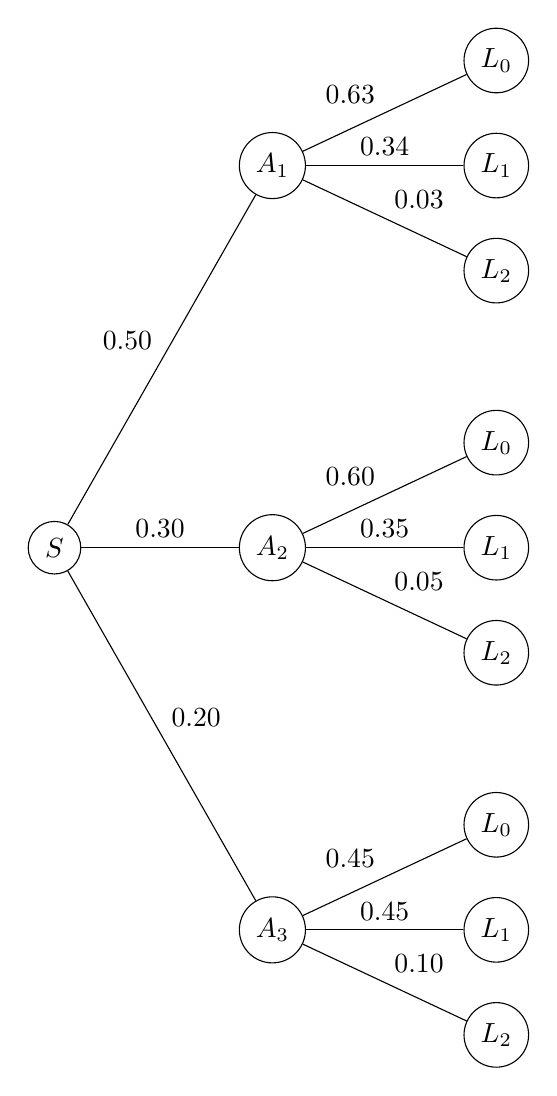
\begin{tikzpicture}
  \node (S) [draw, circle] {\(S\)};
  \node (A2) [draw, circle, right=2 of S] {\(A_2\)};
  \node (A1) [draw, circle, above=4 of A2] {\(A_1\)};
  \node (A3) [draw, circle, below=4 of A2] {\(A_3\)};
  \node (L11) [draw, circle, right=2 of A1] {\(L_1\)};
  \node (L10) [draw, circle, above=0.5 of L11] {\(L_0\)};
  \node (L12) [draw, circle, below=0.5 of L11] {\(L_2\)};
  \node (L21) [draw, circle, right=2 of A2] {\(L_1\)};
  \node (L20) [draw, circle, above=0.5 of L21] {\(L_0\)};
  \node (L22) [draw, circle, below=0.5 of L21] {\(L_2\)};
  \node (L31) [draw, circle, right=2 of A3] {\(L_1\)};
  \node (L30) [draw, circle, above=0.5 of L31] {\(L_0\)};
  \node (L32) [draw, circle, below=0.5 of L31] {\(L_2\)};
  \draw (S) to node [auto] {0.50} (A1);
  \draw (S) to node [auto] {0.30} (A2);
  \draw (S) to node [auto] {0.20} (A3);
  \draw (A1) to node [auto] {0.63} (L10);
  \draw (A1) to node [auto] {0.34} (L11);
  \draw (A1) to node [auto] {0.03} (L12);
  \draw (A2) to node [auto] {0.60} (L20);
  \draw (A2) to node [auto] {0.35} (L21);
  \draw (A2) to node [auto] {0.05} (L22);
  \draw (A3) to node [auto] {0.45} (L30);
  \draw (A3) to node [auto] {0.45} (L31);
  \draw (A3) to node [auto] {0.10} (L32);
\end{tikzpicture}

\begin{gather*}
  P(A_1)P(L_1\mid A_1)=0.5\cdot0.34=0.17 \\
  P(A_2)P(L_1\mid A_2)=0.3\cdot0.35=0.105 \\
  P(A_3)P(L_1\mid A_3)=0.2\cdot0.45=0.09 \\
  \\
  P(L_1)=P(A_1)P(L_1|A_1)+P(A_2)P(L_1|A_2)+P(A_3)P(L_1|A_3)=0.17+0.105+0.09=0.365 \\
  \\
  P(A_1\mid L_1)=\frac{P(A_1)P(L_1\mid A_1)}{P(L_1)}=\frac{0.17}{0.365}=0.466 \\
  P(A_2\mid L_1)=\frac{P(A_2)P(L_1\mid A_2)}{P(L_1)}=\frac{0.105}{0.365}=0.288 \\
  P(A_3\mid L_1)=\frac{P(A_3)P(L_1\mid A_3)}{P(L_1)}=\frac{0.09}{0.365}=0.247
\end{gather*}

\section*{2.71}

An oil exploration company currently has two active projects, one in Asia and the other in Europe.  Let \(A\) be the event
that the Asian project is successful and \(B\) be the event hat the European project is successful.  Suppose \(A\) and \(B\)
are independent events with \(P(A)=0.4\) and \(P(B)=0.7\).

\bigskip

\begin{center}
  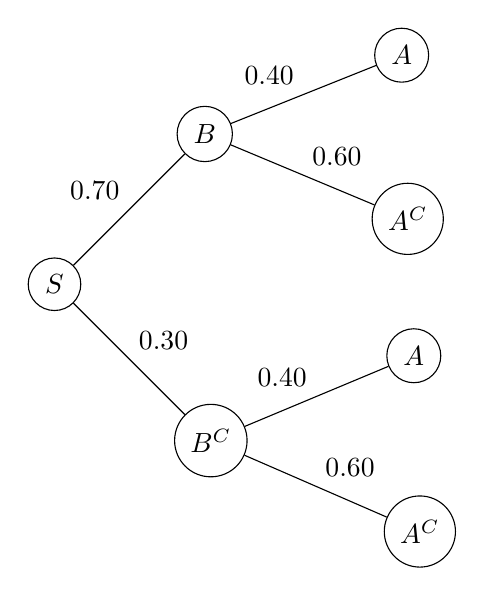
\begin{tikzpicture}
    \node (S) [draw, circle] {\(S\)};
    \node (B) [draw, circle, above right=2 of S] {\(B\)};
    \node (BC) [draw, circle, below right=2 of S] {\(B^C\)};
    \node (AB) [draw, circle, above right=0.5 and 2 of B] {\(A\)};
    \node (ACB) [draw, circle, below right=0.5 and 2 of B] {\(A^C\)};
    \node (ABC) [draw, circle, above right=0.5 and 2 of BC] {\(A\)};
    \node (ACBC) [draw, circle, below right=0.5 and 2 of BC] {\(A^C\)};
    \draw (S) to node [auto] {0.70} (B);
    \draw (S) to node [auto] {0.30} (BC);
    \draw (B) to node [auto] {0.40} (AB);
    \draw (B) to node [auto] {0.60} (ACB);
    \draw (BC) to node [auto] {0.40} (ABC);
    \draw (BC) to node [auto] {0.60} (ACBC);
  \end{tikzpicture}
\end{center}

\bigskip

\begin{enumerate}[label={\alph*)}]
\item If the Asian project is not successful, what its the probability that the European project is also not successful?
  Explain your reasoning.
  \[A\ \text{and}\ B\ \text{independent}\iff A^C\ \text{and}\ B^C\ \text{independent}\]
  \[P(B^C\mid A^C)=P(B^C)=1.00-P(B)=1.00-0.70=0.30\]

\item What is the probability that at least one of the two projects will be successful?
  \begin{align*}
    P(A\cup B) &= P(A)+P(B)-P(A\cap B) \\
    &= P(A)+P(B)-P(A)P(B) \\
    &= 0.4+0.7-0.4\cdot0.7 \\
    &= 0.82
  \end{align*}

\item Given that at least one of the two projects is successful, what is the probability that only the Asian project is
  successful?
  \[P(A\cap B^C)=\frac{0.3\cdot0.4}{0.7+0.3\cdot0.4}=0.146\]
\end{enumerate}

\section*{2.74}

The proportions of blood phenotypes in the U.S. population are as follows:

\begin{tabular}{cccc}
  A & B & AB & O \\
  0.40 & 0.11 & 0.04 & 0.45
\end{tabular}

Assuming that the phenotypes of two randomly selected individuals are independent of one another, what is the probability
that both phenotypes are O?
\[P\left(\text{both O}\right)=0.45\cdot0.45=.203\]
What is the probability that the phenotypes of two randomly selected individuals match?
\[P\left(\text{both match}\right)=0.40\cdot0.40+0.11\cdot0.11+0.04\cdot0.04+0.45\cdot0.45=0.376\]

\section*{2.82}

Consider independently rolling two fair dice, one red and the other green.  Let \(A\) be the event that the red die shows
3 dots, \(B\) be the event that the green die shows 4 dots, and \(C\) be the event that the total number of dots showing on
the two dice is 7.  Are these events pairwise independent (i.e., are \(A\) and \(B\) independent events, are \(A\) and \(C\)
independent events, and are \(B\) and \(C\) independent events)?
\begin{gather*}
  A=\setb{(3,x)}{x=1,2,3,4,5,6} \\
  B=\setb{(x,4)}{x=1,2,3,4,5,6} \\
  C=\set{(1,6),(2,5),(3,4),(4,3),(5,2),(6,1)} \\
  \\
  P(A)=\frac{1}{6} \\
  P(B)=\frac{1}{6} \\
  P(C)=\frac{6}{36}=\frac{1}{6} \\
  \\
  P(A\cap B)=\frac{1}{36}=\frac{1}{6}\cdot\frac{1}{6}=P(A)P(B) \\
  P(A\cap C)=\frac{1}{36}=\frac{1}{6}\cdot\frac{1}{6}=P(A)P(C) \\
  P(B\cap C)=\frac{1}{36}=\frac{1}{6}\cdot\frac{1}{6}=P(B)P(C)
\end{gather*}
Thus, \(A\), \(B\), and \(C\) are pairwise independent.

Are the three events mutually independent?
\begin{gather*}
  P(A\cap B\cap C)=\frac{1}{36} \\
  P(A)P(B)P(C)=\frac{1}{6}\cdot\frac{1}{6}\cdot\frac{1}{6}=\frac{1}{216} \\
  \\
  P(A\cap B\cap C)\ne P(A)P(B)P(C)
\end{gather*}
Thus, \(A\), \(B\), and \(C\) are \emph{not} mutually independent.

\section*{2.84}

Consider purchasing a system of audio components consisting of a receiver, a pair of speakers, and a CD player.  Let \(A_1\)
be the event that the receiver functions properly throughout the warranty period, \(A_2\) be the event that the speakers
function properly throughout the warranty period, and \(A_3\) be the event that the CD play functions properly throughout
the warranty period.  Suppose that these events are (mutually) independent with \(P(A_1)=0.95\), \(P(A_2)=0.98\), and
\(P(A_3)=0.80\).

\begin{enumerate}[label={\alph*)}]
\item What is the probability that all three components function properly throughout the warranty period?
  \[P(A_1\cap A_2\cap A_3)=P(A_1)P(A_2)P(A_3)=0.95\cdot0.98\cdot0.80=0.745\]

\item What is the probability that at least one component needs service during the warranty period?
  \begin{align*}
    P(A_1^C\cup A_2^C\cup A_3^C) &= P\left((A_1\cap A_2\cap A_3)^C\right) \\
    &= 1-P(A_1\cap A_2\cap A_3) \\
    &= 1-0.745 \\
    &= 0.255
  \end{align*}

\item What is the probability that all three components need service during the warranty period?
  \[P(A_1^C\cap A_2^C\cap A_3^C)=P(A_1^C)P(A_2^C)P(A_3^C)=0.05\cdot0.02\cdot0.20=0.0002\]

\item What is the probability that only the receiver needs service during the warranty period?
  \[P(A_1^C\cap A_2\cap A_3)=P(A_1^C)P(A_2)P(A_3)=0.05\cdot0.98\cdot0.80=0.039\]

\item What is the probability that exactly one of the three components needs service during the warranty period?
  \begin{align*}
    P(\text{exactly one}) &= P(A_1^C)P(A_2)P(A_3)+P(A_1)P(A_2^C)P(A_3)+P(A_1)P(A_2)P(A_3^C) \\
    &= 0.05\cdot0.98\cdot0.80+0.95\cdot0.02\cdot0.80+0.95\cdot0.98\cdot0.20 \\
    &= 0.241
  \end{align*}

\item What is the probability that all three components function properly throughout the warranty period but that at least
  one fails within a month after the warranty expires?

  Since we have no data regarding the post-warranty period, any answer would be conjecture.  The best that we can do is
  state that the probability is \(\le0.745\).
\end{enumerate}

\end{document}
